Benchmarking-delens fremmeste formål er at finde svar på en række spørgsmål
inden udregningen sættes igang.  Reelt har vi kun en enkelt parameter vi kan
skrue på, nemlig $m$ - antallet af dronninger vi placerer på hver board før vi
genererer et mig job til at regne videre på det board.  Hvilket forhold mellem 
\fixme{what?}
%\subsection{Takaken}
%\subsection{Java port}
%\subsection{Java port v2}
%\subsubsection{Rekursion vs. Iterativ metode}
%\subsubsection{Iterativ med checkpoints}
%\subsection{MiGrid}

\subsection{Lokale tests}

Vi starter med at teste de forskellige udgaver af koden lokalt, så vi har en
baseline at sammenligne med.

Alle lokale tests er kørt på en IBM T43, med en pentium m 1.86Ghz cpu, 

Java koden er kompilet med javac

\begin{verbatim}
alex@roadrunner:~/temp/queens/src/main/java$ javac -version
javac 1.5.0_11
\end{verbatim}

C koden er kompilet med \texttt{gcc -Os -O2 -o nq nqueens.c}

\begin{verbatim}
alex@roadrunner:~/temp/queens/src/main/java$ gcc --version
gcc (GCC) 4.1.2 (Ubuntu 4.1.2-0ubuntu4)
\end{verbatim}

De første tests er kørt på revision 77 (i forbindelse med den iterative test er
udskrivning af debug info til skærmen dog blevet kommenteret ud)

\begin{figure}[h]
\begin{center}
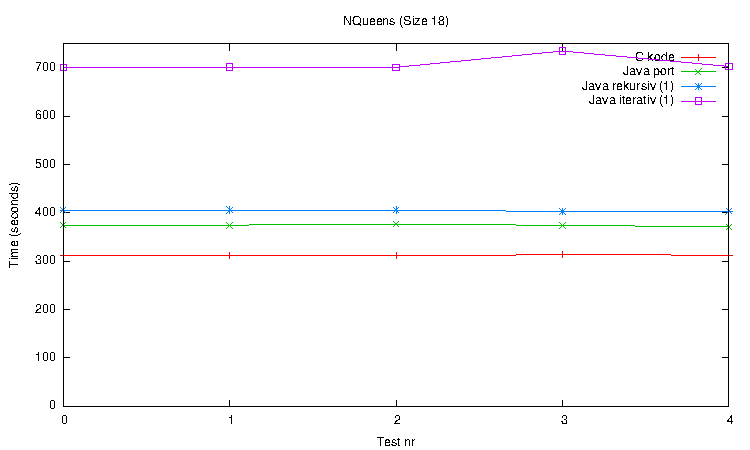
\includegraphics{../benchmarks/b1.pdf}
\caption{insert proper caption here } 
\label{plot:b1}
\end{center}
\end{figure}
\fixme{caption}

Som det ses er C udgaven en smule hurtigere end den direkte java port, der igen
er lidt hurtigere end den paralleliserede udgave af koden, når den kører
rekursivt. Den iterative udgave er væsentlig langsommere..

Den parallelle udgave af koden er i dette tilfælde her kørt med
\texttt{maxSteps} på 1. 

Den næste graf er den rekursive udgave af den parallele kode kørt med forskellig
\texttt{maxSteps}. 

I tabel \ref{tabel:noboards} kan det ses hvor mange boards der bliver genereret
for forskellige $n$ og $maxSteps$. 

\begin{figure}[h]
\begin{center}
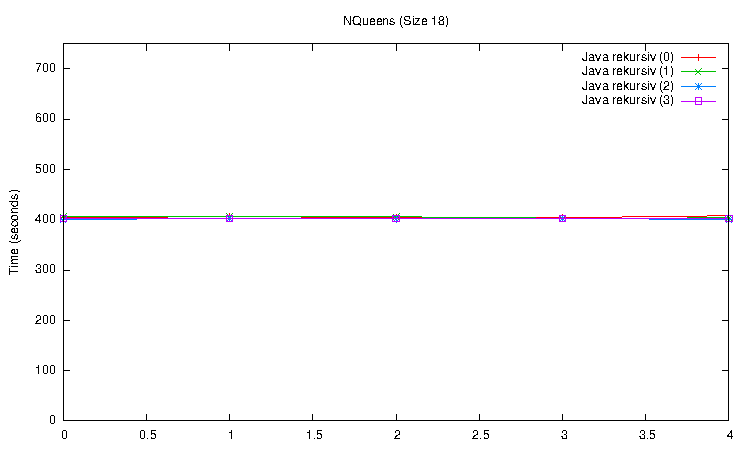
\includegraphics{../benchmarks/b2.pdf}
\caption{insert proper caption here } 
\label{plot:b2}
\end{center}
\end{figure}
\fixme{caption}

Som det ses, har det ikke den store indflydelse på performance, der er altså
ikke det store overhead ved at generere en masse opgaver og løse dem bagefter,
når det kører lokalt. 

Det skal også nævnes at for $maxSteps>n/2$ vil vores program regne forkert.
Dette skyldes \fixme{ja.. hvad skyldes det.. }

\fixme{hvor mange jobs bliver der lavet for de forskellige maxsteps, indsæt
tabel?}
\begin{table}
	\begin{center}
		\begin{tabular}{|c|c|c|c|c|c|}
			\hline N  & maxSteps  & boards & n  & maxSteps & boards \\
			\hline 15 & 0         & 18     & 17 & 0        & 21     \\
			\hline 15 & 1         & 173    & 17 & 1        & 243    \\
			\hline 15 & 2         & 1310   & 17 & 2        & 2282   \\ 
			\hline 15 & 3         & 8349   & 17 & 3        & 18161  \\
			\hline 15 & 4         & 43961  & 18 & 0        & 23     \\
			\hline 16 & 0         & 20     & 18 & 1        & 289    \\
			\hline 16 & 1         & 212    & 18 & 2        & 2983   \\
			\hline 16 & 2         & 1797   & 18 & 3        & 26204  \\
			\hline 16 & 3         & 12840  &    &          &        \\
			\hline 16 & 4         & 76224  &    &          &        \\
			\hline
		\end{tabular}
		\caption{Antal Boards der bliver genereret}
		\label{tabel:noboards}
	\end{center}
\end{table}

Alle tests er i første omgang kørt 5 gange, dette blev gjort for at se om
køretiden svingede meget, da dette ikke lader til at være tilfældet vil resten
af testene kun blive kørt 1 gang.. 

Nu skal vi så se på hvor hurtigt det kører når vi smider det efter MiGrid. 
Disse tests er kørt med \texttt{maxSteps} 0 og 1.

\fixme{indsaet en graf, eller bare resultaterne og henvis til b3?}
De foregående tests er kørt med kode der bruger \texttt{int} til at gemme resultaterne,
i de næste tests er \texttt{int} skiftet ud med \texttt{BigInteger} (revision
83
\clearpage
Sammenligning af alle benchmarks

\begin{figure}[h]
\begin{center}
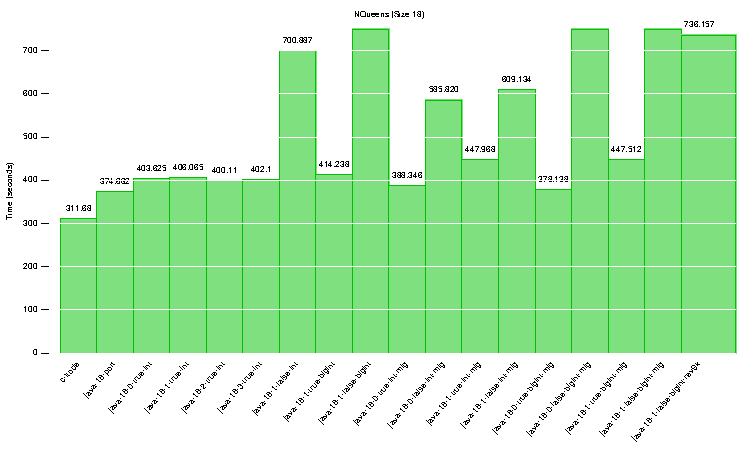
\includegraphics{../benchmarks/b3.pdf}
\caption{nsert proper caption here } 
\label{plot:b3}
\end{center}
\end{figure}
\fixme{caption}

Som det ses på figur \ref{plot:b3} kører den iterative udgave af koden fra
rev. 83 utroligt langsomt i forhold til foregående udgaver. 
Dette skyldes en en linje kode, der ikke var blevet kommenteret ud. Denne linje
konkatenerede to strenge. Uden denne linje kører koden væsentlig hurtigere, som
det ses af søjle 18. Den rekursive kode kører en smule langsommere med
\texttt{BigInteger} (søjle 4 mod søjle 8), hvor tiden stiger fra 406.xxx til
414.xxx\fixme{indsaet rigtige tal}, hvilket svarer til en forøgelse på knap 2\%

\begin{itemize}
\item[1] Takakens C-kode
\item[2] Direkte java port
\item[3] Parallel java port, \texttt{maxSteps}=0, rekursiv, int, lokal
\item[4] Parallel java port, \texttt{maxSteps}=1, rekursiv, int, lokal
\item[5] Parallel java port, \texttt{maxSteps}=2, rekursiv, int, lokal
\item[6] Parallel java port, \texttt{maxSteps}=3, rekursiv, int, lokal
\item[7] Parallel java port, \texttt{maxSteps}=1, iterativ, int, lokal
\item[8] Parallel java port, \texttt{maxSteps}=1, rekursiv, bigint, lokal
\item[9] Parallel java port, \texttt{maxSteps}=1, iterativ, bigint, lokal
\item[10] Parallel java port, \texttt{maxSteps}=0, rekursiv, int, MiG
\item[11], Parallel java port, \texttt{maxSteps}=0, iterativ, int MiG
\item[12], Parallel java port, \texttt{maxSteps}=1, rekursiv, int, MiG
\item[13], Parallel java port, \texttt{maxSteps}=1, iterativ, int, MiG
\item[14], Parallel java port, \texttt{maxSteps}=0, rekursiv, bigint, MiG
\item[15], Parallel java port, \texttt{maxSteps}=0, iterativ, bigint, MiG
\item[16], Parallel java port, \texttt{maxSteps}=1, rekursiv, bigint, MiG
\item[17], Parallel java port, \texttt{maxSteps}=1, iterativ, bigint, MiG
\item[18], Parallel java port, \texttt{maxSteps}=1, iterativ, bigint, rev107 
\fixme{indsaet sidste tests her og opdatere graph}
\end{itemize}

\subsection{overhead ved jobskifte}

I MiG\_main() metoden i NQueenJob laver vi et timestamp i starten og slutningen af metoden. 
og kan så tage start tiden for et job og trække sluttiden for det foregående job
fra, og man har så et estimat for hvor lang tid et jobskifte tager, vi har gjort
dette for 8 jobs, og får så 7 estimater, gennemsnittet af dem bliver 18.455 sek. 
Op til 15 af disse 18 sekunder, skyldes at oneclick applet'en sover i 15 sekunder. 
Ved en kørsel med $n=18$ og $maxSteps=1$, hvor vi så får 289 jobs, giver det
knap 89 minutter. 

\subsection{kald til backtrack}
Hvis man ser på antallet af kald til backtrack de forskellige versioner laver, er de
ens for c koden og den direkte java port, og hvis man kører med $maxSteps=0$ er
antallet af kald for den parallele og iterative kode også det samme som
for c koden. Med $maxSteps>0$ får vi færre kald til backtrack, hvilket skyldes
at en del af disse kald bliver lavet i forbindelse med oprettelsen af de ekstra
boards. 

\begin{table}
\begin{center}
\begin{tabular}{|c|c|c|c|c|c|c|c|}
\hline N  & kodebase 		  & middleboard & cornerboard & N  & kodebase      & middleboard & cornerboard \\
\hline 15 & C kode   			&             &             & 17 & C kode        &             &             \\
\hline 15 & Java          &             &             & 17 & Java          &             &             \\
\hline 15 & Java rek. &             &             & 17 & Java rek. &             &             \\
\hline 15 & Java ite. &             &             & 17 & Java ite. &             &             \\
\hline 16 & C kode   			&             &             & 18 & C kode        &             &             \\
\hline 16 & Java          &             &             & 18 & Java          &             &             \\
\hline 16 & Java rek. &             &             & 18 & Java rek. &             &             \\
\hline 16 & Java ite. &             &             & 18 & Java ite. &             &             \\
\hline
\end{tabular}
\caption{Kald til backtrack}
\label{table:backtrackkald}
\end{center}
\end{table}
\fixme{indsæt tal (*07-01*)}

\subsection{Jobstørrelse}

Med jobstørrelse refererer vi til hvor lang tid det tager at løse et job, og
ikke størrelsen på data. 
Som det ses i \ref{tabel:jobsize}, varierer jobstørrelsen
meget. Cornerboards er generelt ret små, mens middleboards er generelt er en del
større. Det ses også i tabellen at jobstørrelsen afhænger af de bounds der er i
henholdsvist MiddleBoard og CornerBoard. Hvis man øger $maxSteps$ og dermed får
lavet flere jobs, ses det at de enkelte jobs bliver delt op i nogenlunde lige
støre dele, den relative størrelse mellem det mindste og største jobs er dog
stadig nogenlunde det samme. \fixme{lav en benchmark/beregning der viser dette?}

\subsection{Generering af jobs}

Generering og indsendelse af jobs afhænger tildels af den internetforbindelse
man sidder på, da indsendelse jo går via internettet. De forskellige jobs vi har
submitted til MiGrid har genereringen og indsendelse af jobs svinget fra xx til
xx (se tabel \ref{tabel:jobgenerering}) \fixme{lav den fscking tabel og skriv de
rigtige tal ind}. Langt den største del af tiden går også med at sende jobsne,
da genereringen af jobs for større mængder jobs tager ca 0.01ms/job
\begin{verbatim}
18: 4, 6, 44, 280
18: 23, 289, 2983, 26204
18: 0.17, 0.02, 0.01, 0.01
17: 4, 6, 23, 206, 1252
17: 21, 243, 2282, 18161, 121116
17: 0.19, 0.02, 0.01, 0.01, 0.01
\end{verbatim}
\fixme{lav det om til en tabel.. der}
